\label{capitolo1}
\section{Introduzione}
A partire dalla metà degli anni '80, grazie a due innovazioni tecnologiche si fecero diversi passi avanti nell'uso dei calcolatori. La prima di queste innovazioni fu lo sviluppo di microprocessori potenti; la seconda grande innovazione fu l'invenzione delle reti di computer con l'introduzione delle \textbf{LAN} (\emph{Local Area Network}) che consentirono a centinaia di macchine di essere connesse le une alle altre e permisero lo scambio di piccole quantità di informazioni in pochi microsecondi.\\
Il risultato di questa innovazione tecnologica è che oggi mettere insieme una grande quantità di computer tramite una rete ad alta velocità è diventato molto semplice. Questo tipo di sistemi sono solitamente chiamate \emph{reti di computer} o \textbf{sistemi distribuiti}.
\subsection{Definizione di sistema distribuito}
Esistono diverse definizioni di \emph{Sistema distribuito} ma tutte quante sono abbastanza insoddisfacenti. Daremo ora una prima definizione che è sufficente per i nostri scopi:
\begin{center}
\emph{Un sistema distribuito è una collezione di computer indipendenti che appare ai propri utenti come un singolo sistema coerente}
\end{center}
Da questa definizione possiamo ricavare diversi caratteristiche di un sistema distribuito, la prima è che i sistemi distribuiti sono costituiti da componenti autonomi; la seconda è che gli utenti, siano essi persone o altri programmi, vedono il sistema come un'unica entità. Il che significa che i diversi componenti devono in qualche modo collaborare.\\
Quello che non viene specificato in questa definizione è il tipo di computer usati per i componenti ne come questi sono interconnessi.\\
Le caratteristiche più importanti dei sistemi distribuiti sono il fatto che le differenze tra i vari computer e le loro modalità di comunicazione risultano per lo più nascoste agli utenti finali. Inoltre gli utenti possono interagire con un sistema distribuito in modo \emph{consistente} e \emph{uniforme} ovvero indipendentemente da dove e quando avviene l'interazione.\\
Teoricamente i sistemi distribuiti dovrebbero essere facilmente espandibili e scalabili, inoltre, i sistemi distribuiti sono di norma sempre disponibili anche se alcune sui parti sono momentaneamente fuori uso.\\
Allo scopo di supportare reti eterogenee e sistemi operativi differenti alle volte si introduce uno strato software tra lo strato di applicazione e i diversi sistemi operativi, questo strato è chiamato \textbf{middleware} come mostrato in figura \ref{fig:midd}.
\begin{figure}[htb]
\centering
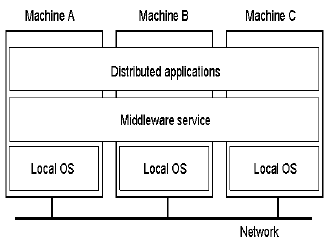
\includegraphics[width=8cm]{img/schemamidd.png}\\
\caption{Schema di un middleware}\label{fig:midd}
\end{figure}
\subsection{Obiettivi}
La possibilità costruire sistemi distribuiti non implica che tutti i sistemi debbano essere costruiti come sistemi distribuiti. Per far si che sia utile progettare e costruire un sistema distribuito dobbiamo rispettare alcune caratteristiche. un sistema distribuito dovrebbe:
\begin{itemize}
\item rendere le risorse facilmente accessibili,
\item nascondere il fatto che le risorse sono distribuite sulla rete,
\item essere aperto,
\item essere scalabile.
\end{itemize}
\subsubsection{Accessibilità delle risorse}
L'obiettivo principale di un sistema distribuito è quello di rendere facile l'accesso alle risorse remote e condividerle in maniera efficiente e controllata.\\
Ma che cosa intendiamo per "risorse"? Con il termine \emph{risorse} possiamo indicare qualsiasi cosa, alcuni esempi tipici sono stampanti, computer, dati, file, pagine web o intere reti.
Le ragioni che portano a voler condividere le risorse sono molteplici, la prima è sicuramente quella economica, pensiamo ad esempio a ricercatori che condividono un supercomputer o ad una stampante condivisa in un ufficio. Inoltre, la connessione di più utenti facilita la collaborazione come avviene nei \textbf{groupware} dove gruppi di persone lavorano insieme anche stando in diverse parti del mondo.\\
Tutto questo incremento di connessione e collaborazione porta però ad una necessaria crescita anche in termini di sicurezza.